\documentclass[10pt]{beamer} 
\usepackage[utf8]{inputenc}
\usepackage[T1]{fontenc}
\usepackage[spanish]{babel}
\usepackage{mathtools}
\usepackage{utopia} % fuente Utopia
\usetheme{CambridgeUS}
\usecolortheme{dolphin}

%================== Colores ==================% 
\usepackage[table]{xcolor} 
\definecolor{lavanda}{HTML}{B8A9C9}
\definecolor{lavandaClaro}{HTML}{F5F2FA}
\definecolor{ink}{HTML}{222222}
\colorlet{Accent}{lavanda}
\colorlet{AccentSoft}{lavandaClaro}
\colorlet{Ink}{ink}

%------------------------------------------------------------
% Colores lavanda en el tema Beamer
%------------------------------------------------------------
\setbeamercolor*{palette primary}{bg=AccentSoft, fg=Ink}   % barra clara
\setbeamercolor*{palette secondary}{bg=Accent,    fg=white}
\setbeamercolor*{palette tertiary}{bg=Accent,    fg=white}

\setbeamercolor*{titlelike}{fg=Accent}
\setbeamercolor*{title}{bg=Accent, fg=white}
\setbeamercolor*{item}{fg=Accent}
\setbeamercolor*{caption name}{fg=Accent}
\setbeamercolor*{frametitle}{fg=Accent}
\setbeamercolor*{normal text}{fg=Ink, bg=white}

\usefonttheme{professionalfonts}

\usepackage{hyperref}
\usepackage{natbib}
\usepackage{graphicx}
\graphicspath{{../Figures/}}
\usepackage{tikz}
\usetikzlibrary{positioning}



%------------------------------------------------------------
% Datos de la presentación
%------------------------------------------------------------
\setbeamerfont{title}{size=\large}
\setbeamerfont{subtitle}{size=\small}
\setbeamerfont{author}{size=\small}
\setbeamerfont{date}{size=\small}
\setbeamerfont{institute}{size=\small}

\title[Segmentación por endeudamiento]{Segmentación de Clientes por Perfil de Endeudamiento}
\subtitle{Aprendizaje no supervisado}
\author[Debany Hernández]{Debany Jazmín Hernández Camacho}
\institute[CIMAT]{Maestría en Matemáticas Aplicadas \\ Centro de Investigación en Matemáticas (CIMAT) \\ debany.hernandez@gmail.com}
\date[Proyecto final]{Introducción a la Ciencia de Datos \\ Proyecto Final}

%------------------------------------------------------------
% Diapositiva de transición al inicio de cada sección
%------------------------------------------------------------
\AtBeginSection[]{
  \begin{frame}
  \vfill
  \centering
  \begin{beamercolorbox}[sep=8pt,center,shadow=true,rounded=true]{title}
    \usebeamerfont{title}\insertsectionhead\par%
  \end{beamercolorbox}
  \vfill
  \end{frame}
}

%------------------------------------------------------------
\begin{document}

%==================== Portada ====================%
\frame{\titlepage}


%=================== Introducción =====================%
\section{Introducción}
\begin{frame}{ \textbf{Introducción}}
La segmentación de clientes es una herramienta central en el análisis moderno de datos financieros,
pues permite distinguir entre individuos con bajo riesgo, perfiles estables y usuarios con mayor
probabilidad de presentar dificultades en el pago de sus obligaciones.

\vspace{0.3cm}

En la práctica, cada cliente combina distintos niveles de:
\begin{itemize}
    \item ingreso,
    \item uso del crédito,
    \item historial de morosidad,
    \item carga financiera y número de dependientes.
\end{itemize}

Esta heterogeneidad hace insuficiente cualquier clasificación basada en pocas variables o reglas
simples, y motiva el uso de métodos estadísticos capaces de descubrir estructuras más complejas
directamente a partir de los datos.
\end{frame}


\begin{frame}{\textbf{Planteamiento del problema }}
Se trabajó con la base de datos \textit{Give Me Some Credit}, que recopila información
financiera y demográfica de aproximadamente 150{,}000 clientes. Cada registro resume la situación
crediticia de un cliente mediante variables relacionadas con ingreso, endeudamiento, uso del crédito
y comportamiento de pago.

\vspace{0.3cm}

\textbf{Objetivo}
\begin{itemize}
    \item Identificar, sin etiquetas previas, \textbf{perfiles homogéneos de clientes} a partir de sus
    características crediticias.
\end{itemize}

\textbf{Preguntas guía}
\begin{itemize}
    \item ¿Qué caracteriza a los clientes menos riesgosos?
    \item ¿Qué patrones de endeudamiento o morosidad distinguen los grupos más vulnerables?
    \item ¿Cómo se relacionan variables como ingresos, utilización de crédito y número de dependientes con el 
    comportamiento crediticio?
\end{itemize}
\end{frame}

\section{Metodología}
\begin{frame}

La base de datos \textit{Give Me Some Credit} contiene 10 variables financieras y demográficas
relacionadas con endeudamiento, ingreso y comportamiento de pago.

\vspace{0.3cm}

\small
\rowcolors{2}{AccentSoft}{white}
\setlength{\tabcolsep}{6pt}
\renewcommand{\arraystretch}{1.2}

\begin{table}[H]
\centering
\begin{tabular}{p{4cm} p{6.5cm}}
\rowcolor{Accent!40}
\textbf{Variable} & \textbf{Descripción} \\

RevolvingUtilizationOfUnsecuredLines & Uso relativo de líneas de crédito no aseguradas. \\

age & Edad del cliente. \\

DebtRatio & Proporción entre gastos + pagos de deuda y el ingreso mensual. \\

MonthlyIncome & Ingreso mensual declarado. \\

NumberOfOpenCreditLinesAndLoans & Número total de cuentas y préstamos activos. \\

NumberRealEstateLoansOrLines & Préstamos o líneas inmobiliarias (ej. hipotecas). \\

NumberOfDependents & Número de dependientes económicos. \\

NumberOfTime30--59DaysPastDueNotWorse & Atrasos de 30–59 días. \\

NumberOfTime60--89DaysPastDueNotWorse & Atrasos de 60–89 días. \\

NumberOfTimes90DaysLate & Atrasos graves (90+ días). \\

\end{tabular}
\end{table}

\end{frame}

\begin{frame}{\textbf{Preprocesamiento}}

Antes de aplicar técnicas de aprendizaje no supervisado, se realizó un
preprocesamiento para asegurar que las variables fueran comparables y
estables.

\vspace{0.35cm}

\textbf{Pasos principales:}
\begin{itemize}
    \item Eliminación de registros duplicados y del caso con edad igual a 0.
    \item Imputación de valores faltantes:
    \begin{itemize}
        \item \textit{MonthlyIncome}: mediana (distribución altamente asimétrica).
        \item \textit{NumberOfDependents}: moda.
    \end{itemize}
    \item Winsorización de outliers severos en:
    \begin{itemize}
        \item \textit{RevolvingUtilizationOfUnsecuredLines} (percentil 99).
        \item \textit{DebtRatio} (percentil 99.5).
    \end{itemize}
    \item Estandarización de todas las variables usando \texttt{StandardScaler}.
\end{itemize}

\end{frame}

\begin{frame}{\textbf{Reducción de dimensionalidad (PCA)}}

\begin{itemize}
    \item Aplicamos PCA sobre las 10 variables estandarizadas.
    \item Los primeros \textbf{6 componentes} explican $\approx \textbf{87.6\%}$ de la varianza.
\end{itemize}

\vspace{0.4cm}
\centering
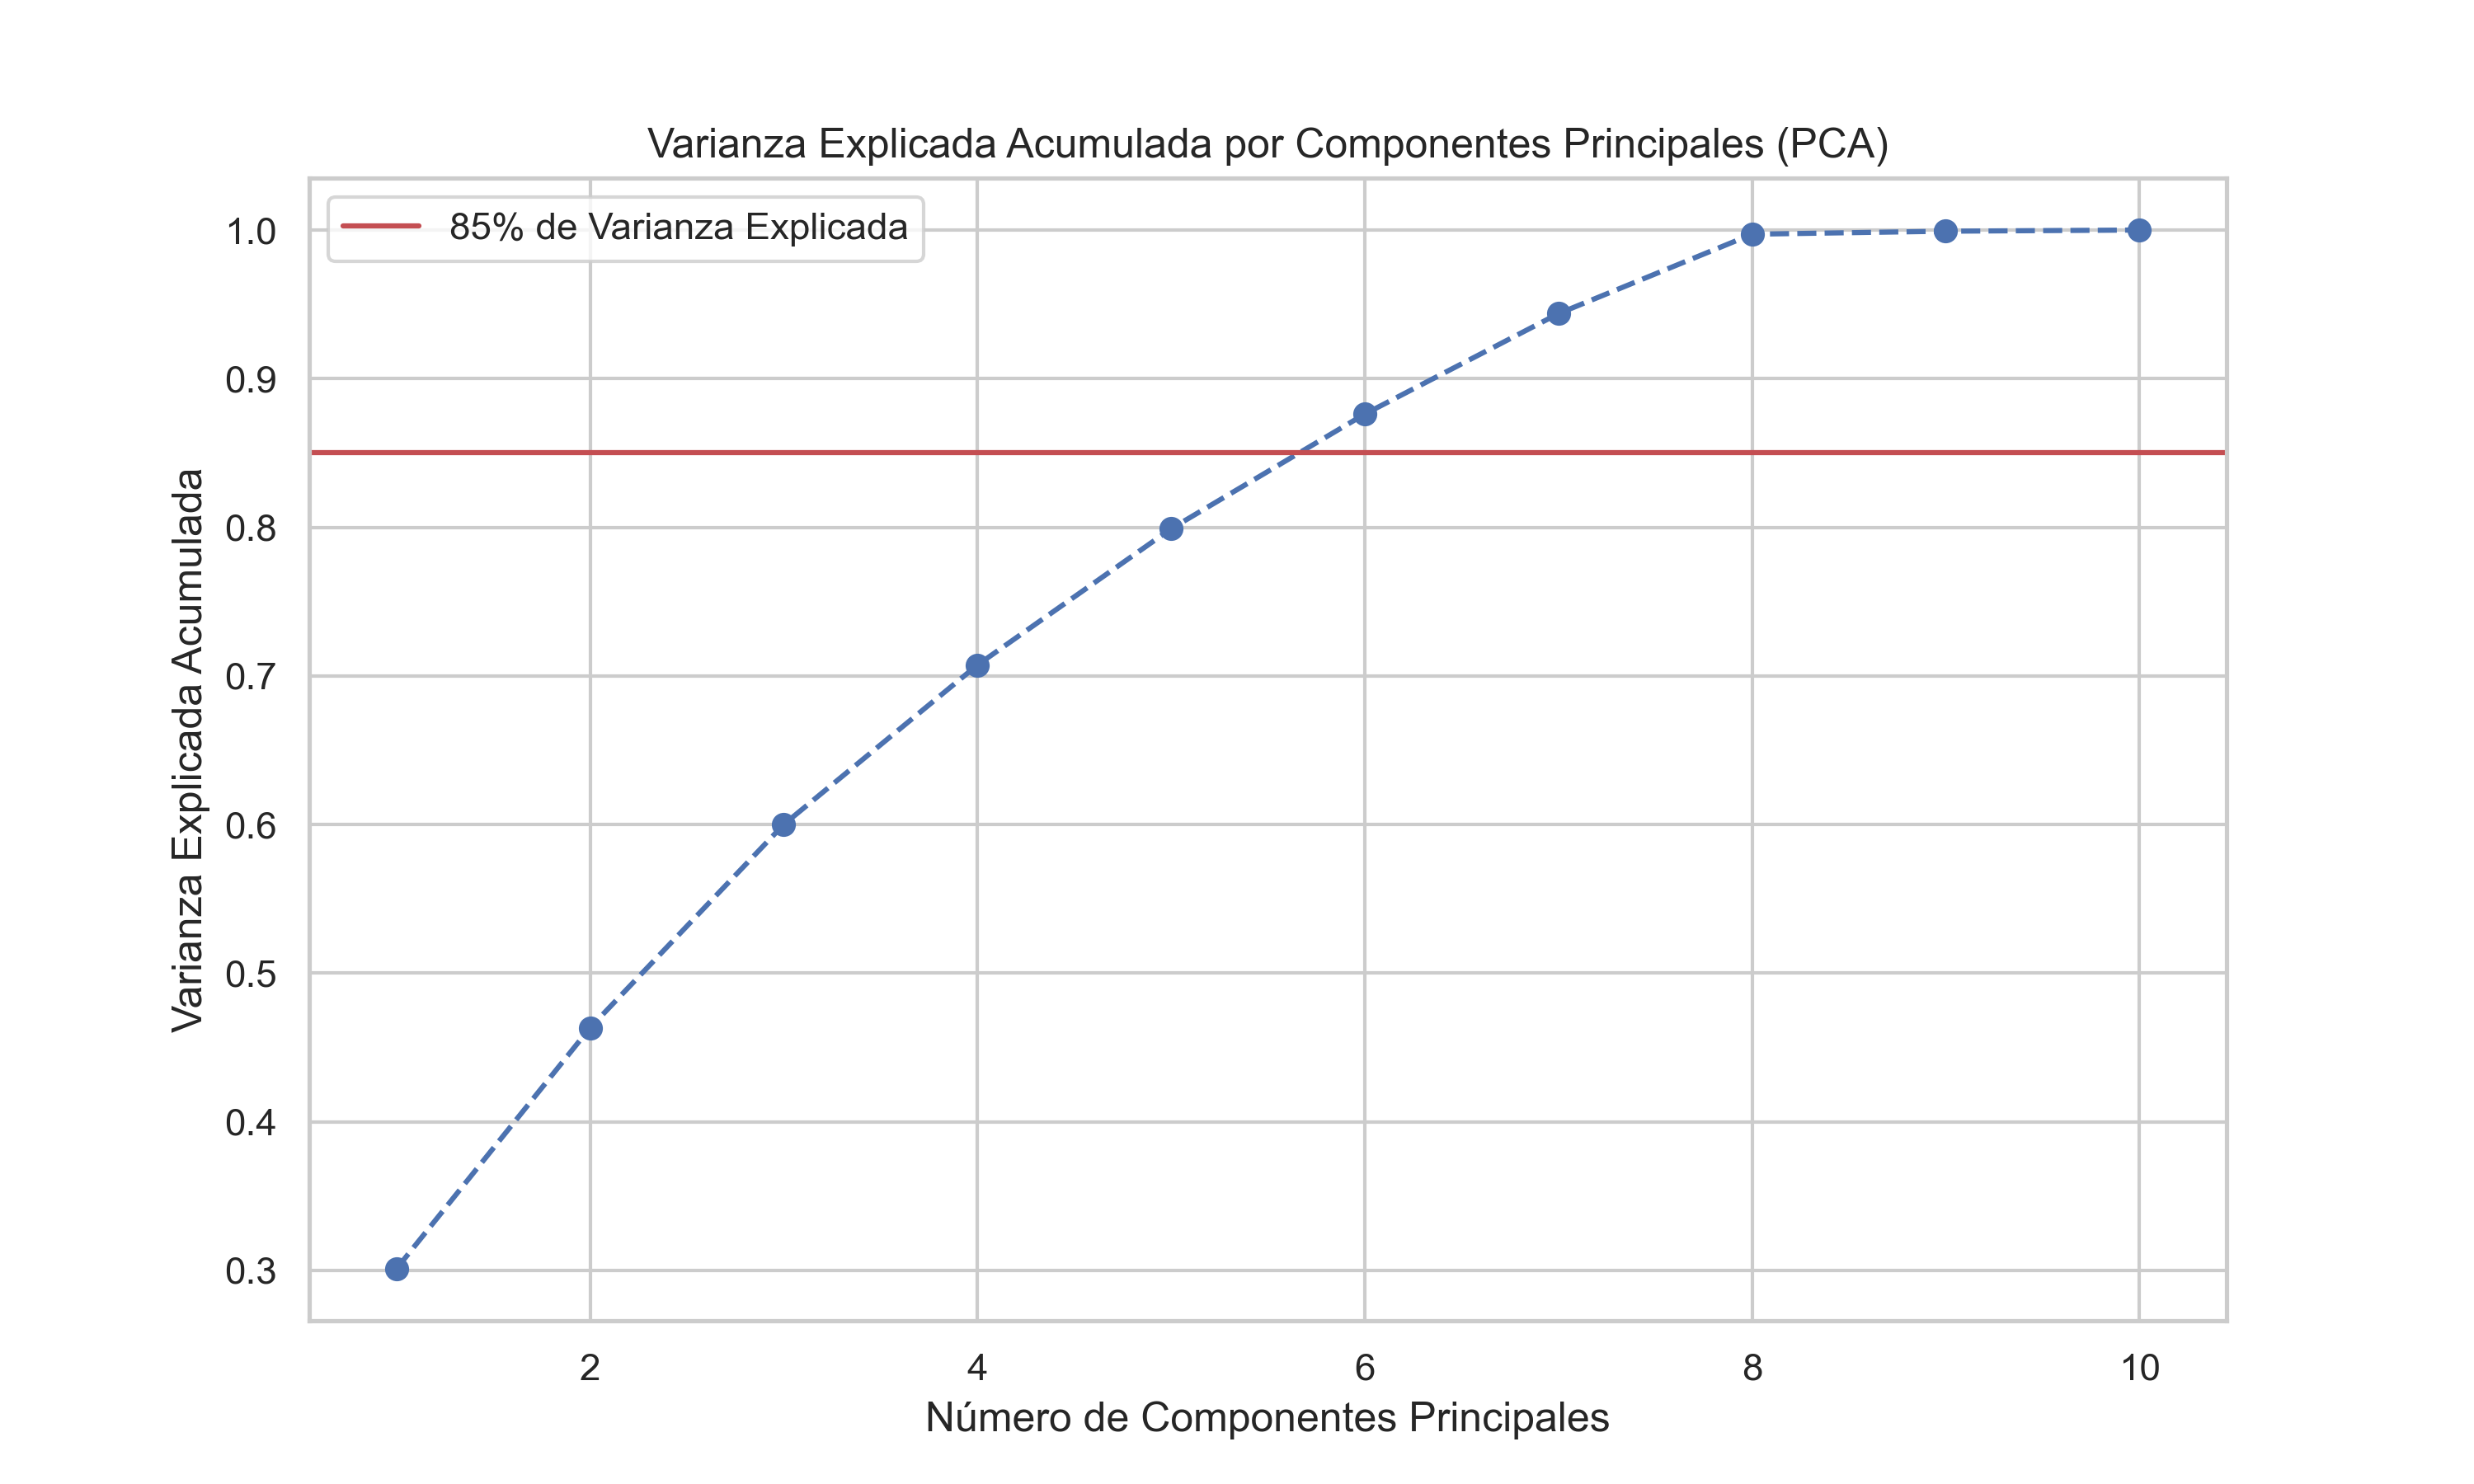
\includegraphics[width=0.8\textwidth]{varianza_explicada_pca.png}

\end{frame}

\begin{frame}{\textbf{Selección del número de clusters (K-Means)}}

\begin{itemize}
    \item Se evaluaron $k = 2$ a $10$ con dos criterios: método del codo y coeficiente de silhouette.
    \item Se seleccionó \textbf{$k = 5$} por estabilidad e interpretabilidad.
\end{itemize}

\vspace{0.4cm}

\begin{columns}[T]
\column{0.5\textwidth}
\centering
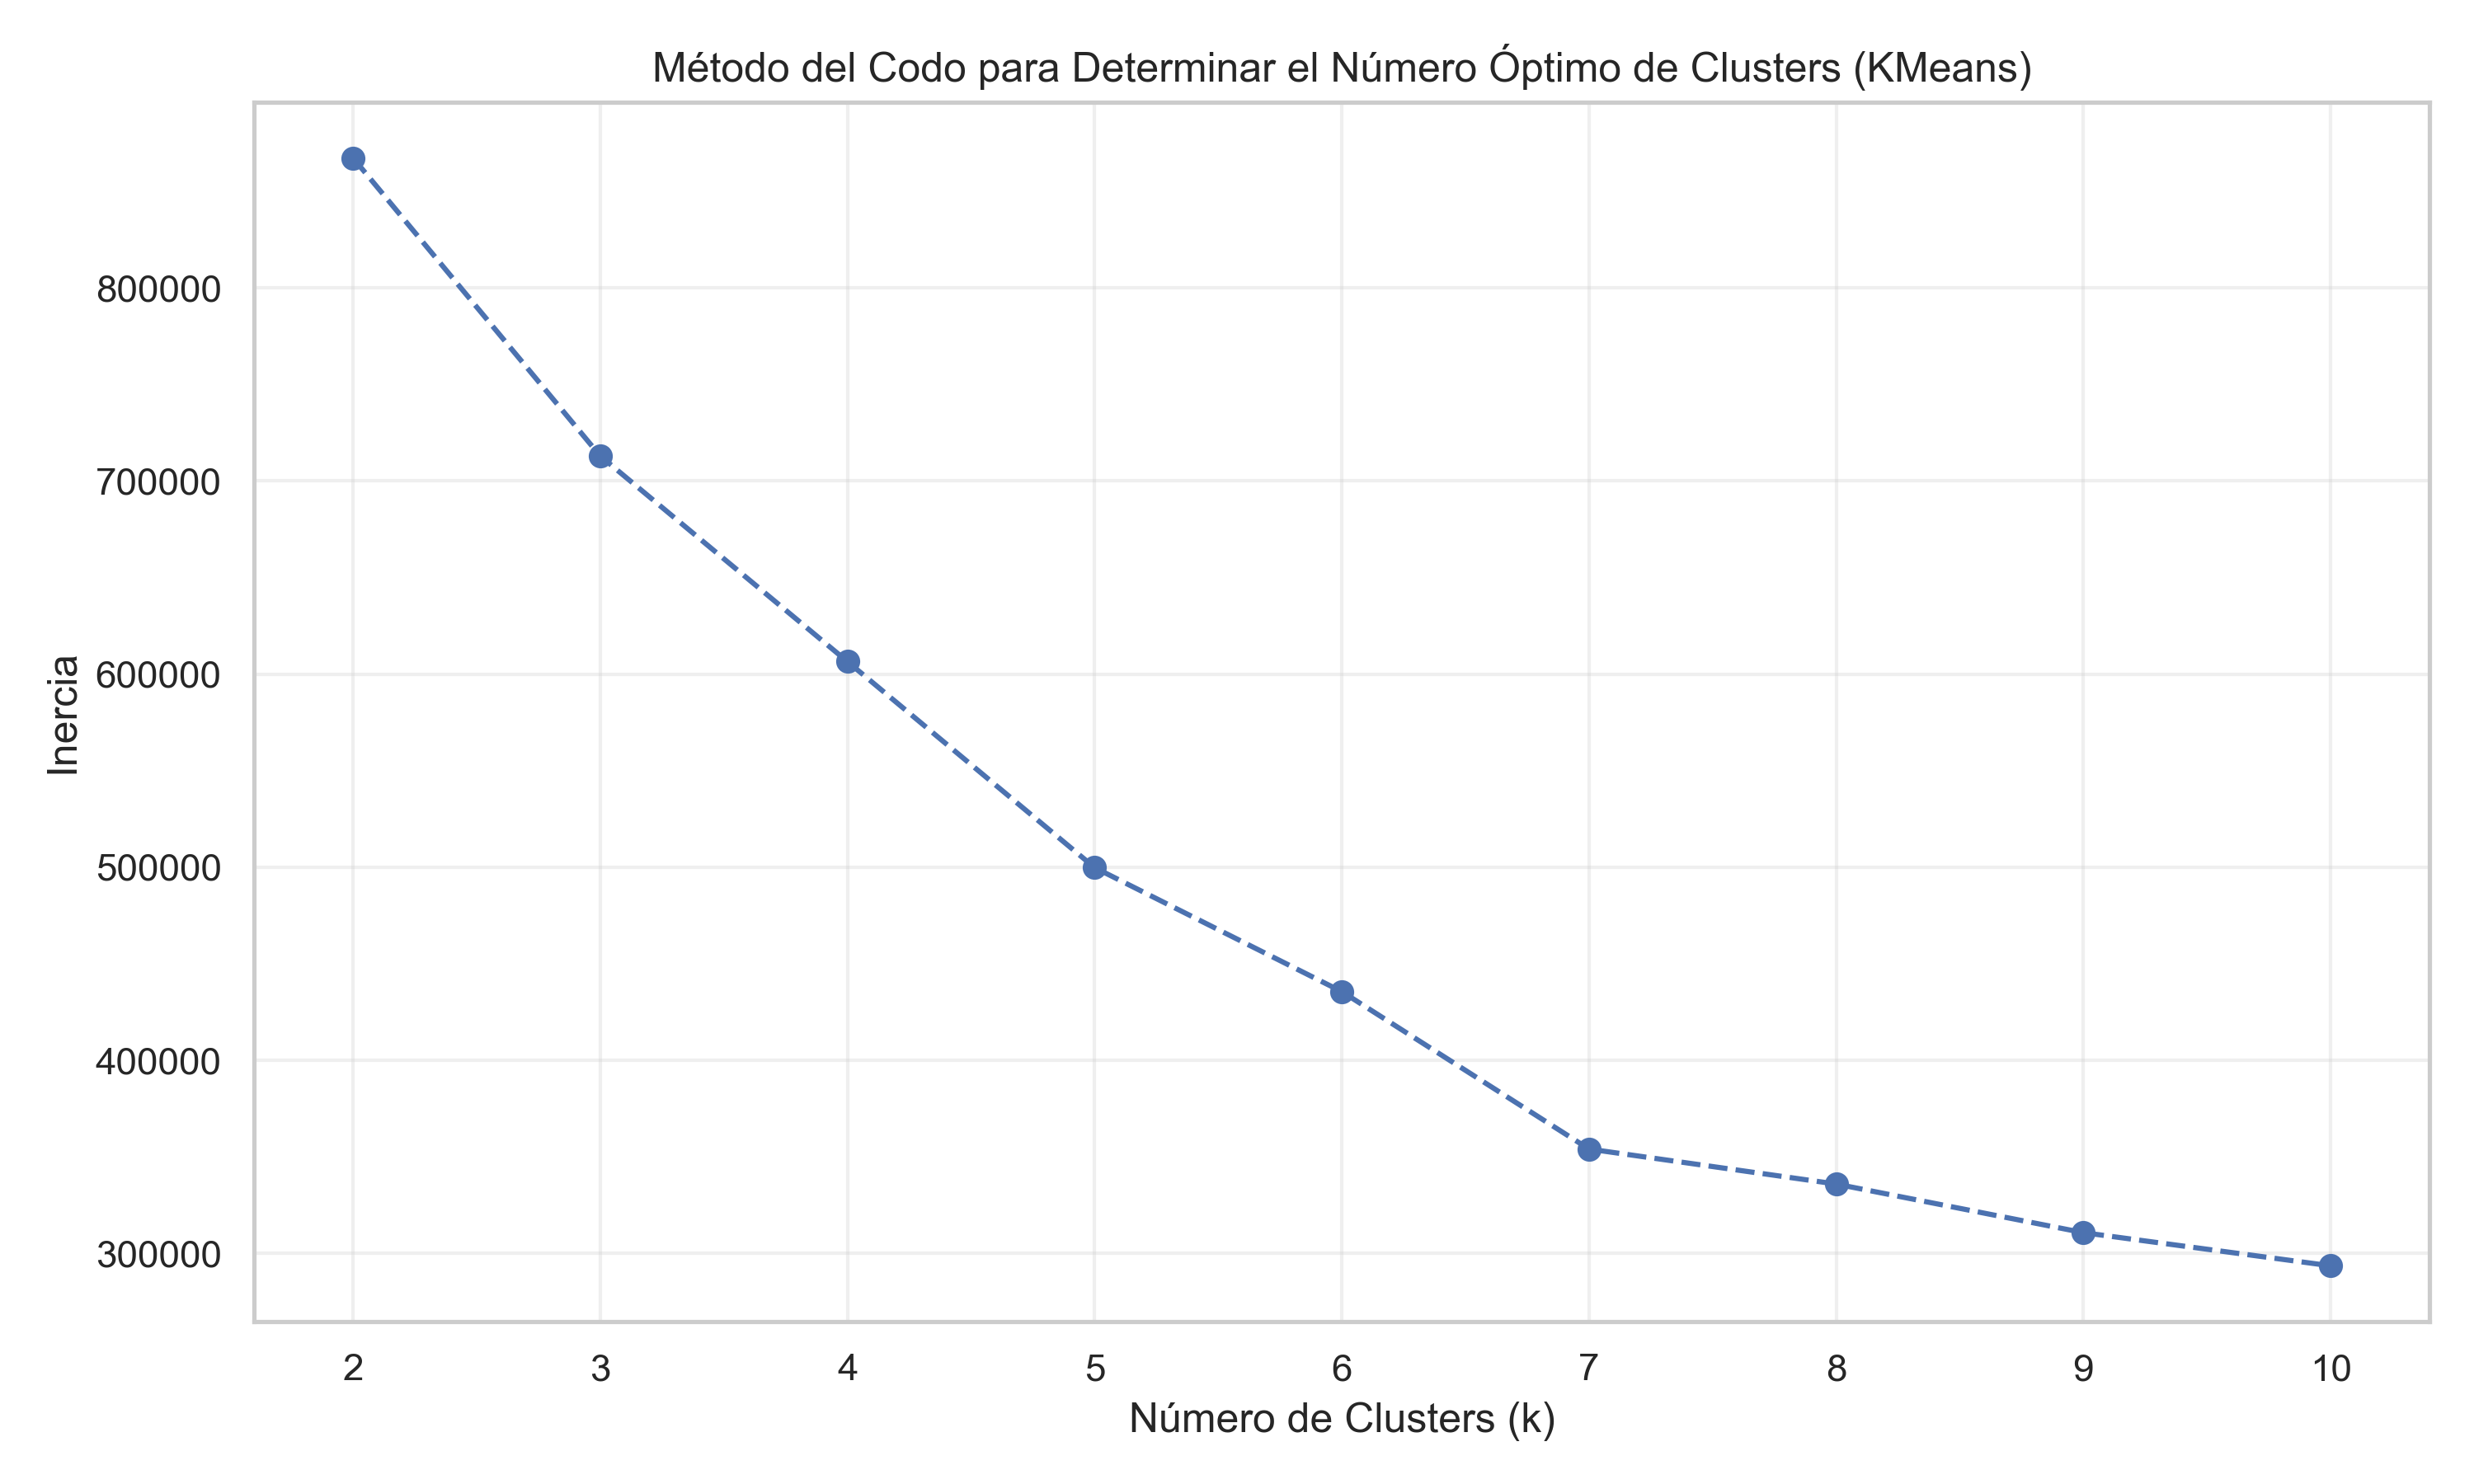
\includegraphics[width=\textwidth]{metodo_del_codo_kmeans.png}

\column{0.5\textwidth}
\centering
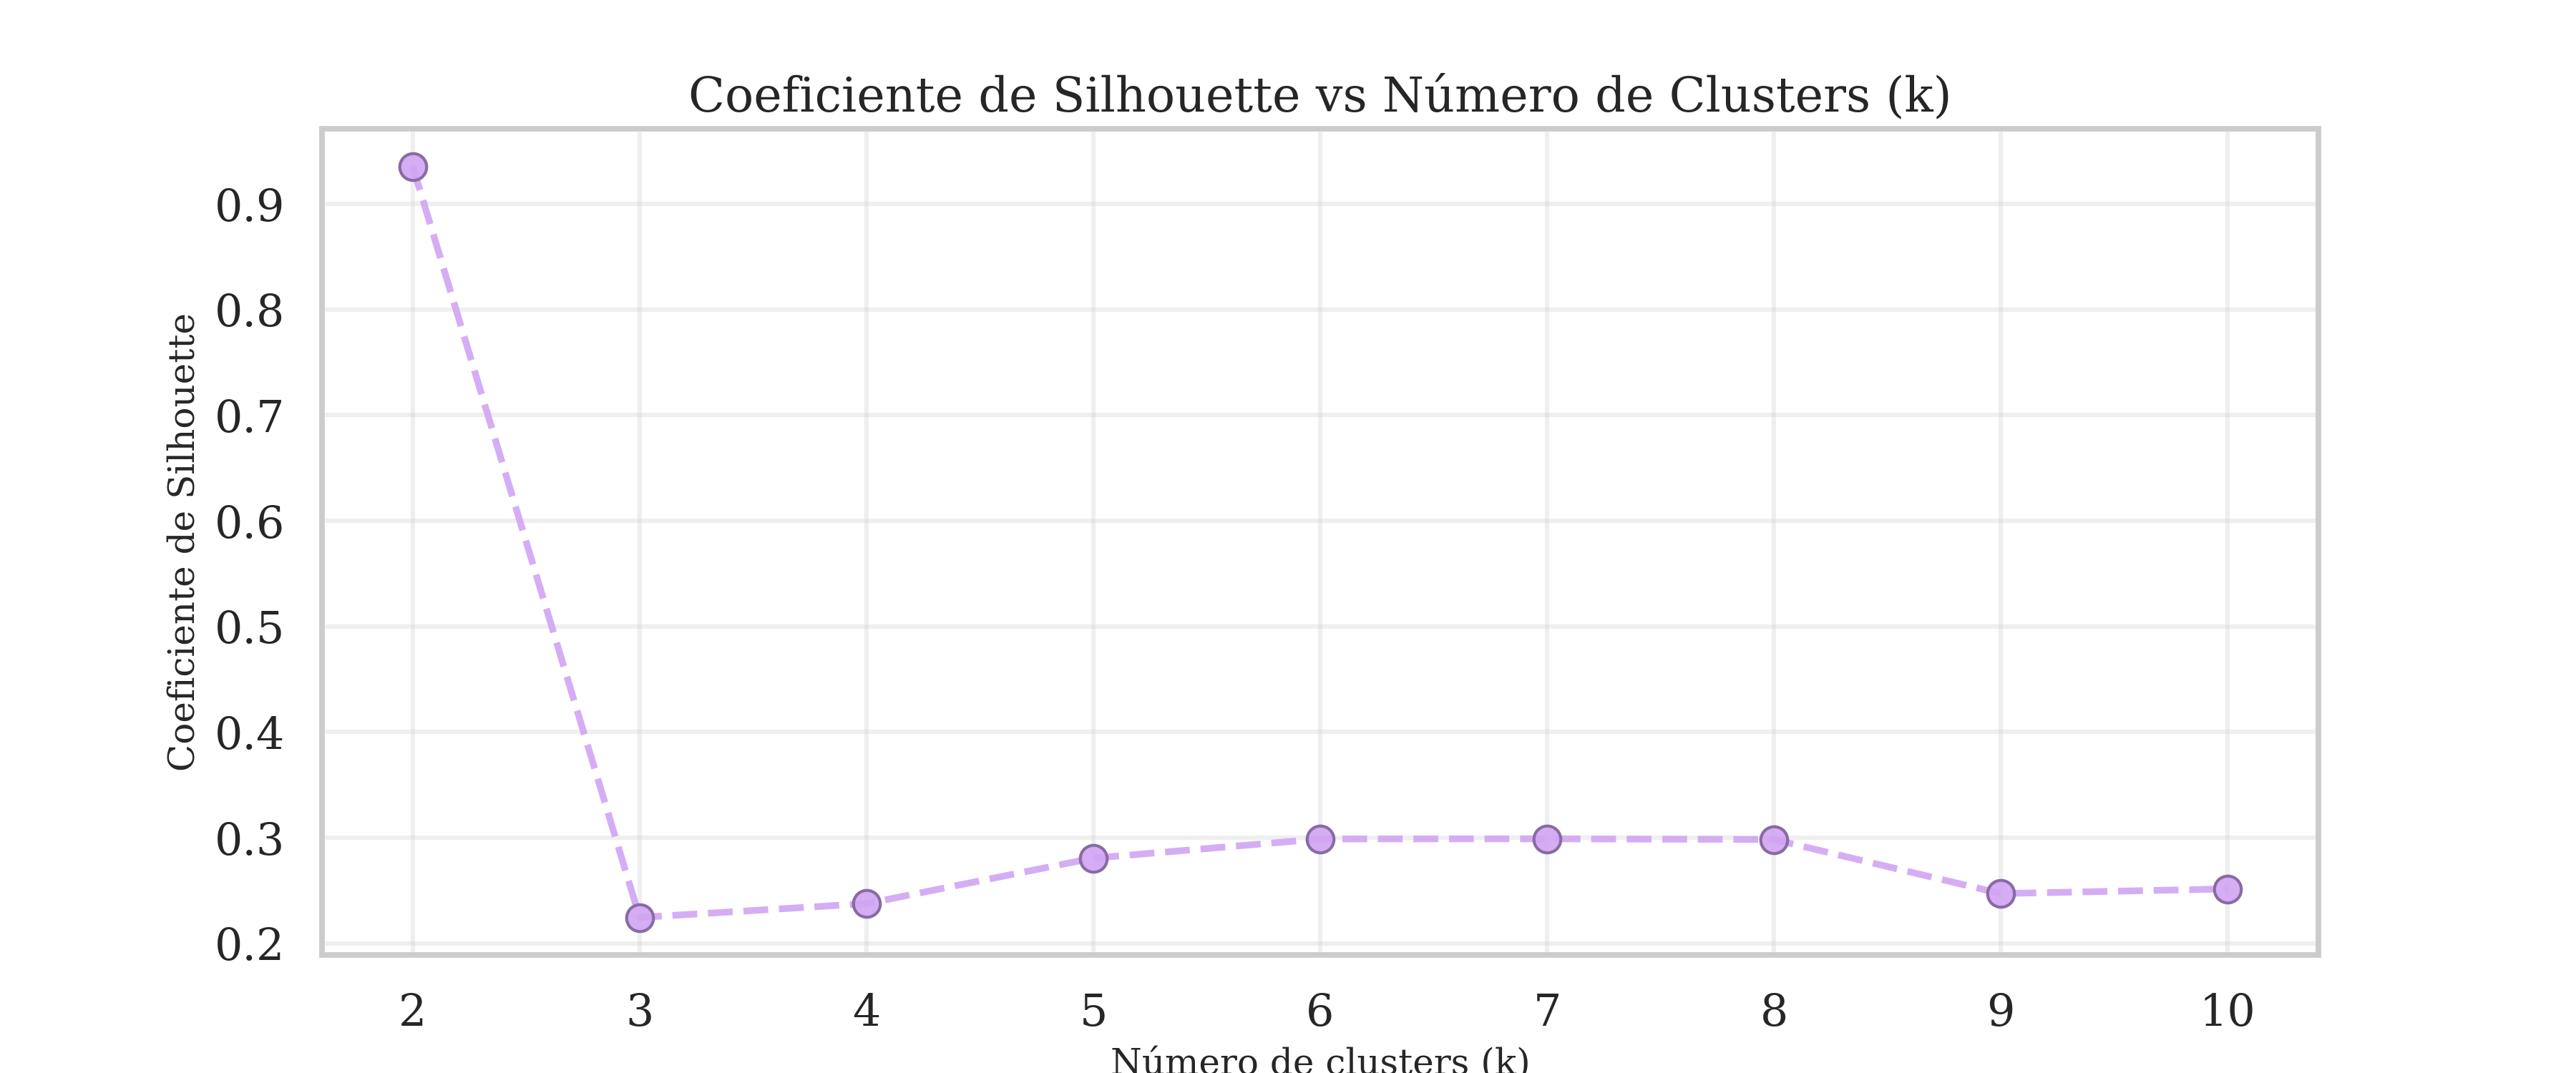
\includegraphics[width=\textwidth]{silhouette_vs_k_kmeans.png}

\end{columns}

\end{frame}
\section{Resultados}
\begin{frame}{\textbf{Resultados principales}}

La tabla resume las medias de cada variable agrupadas por temática para los 5 clusters.

\vspace{0.35cm}

\small
\rowcolors{2}{AccentSoft}{white}
\setlength{\tabcolsep}{3.5pt}
\renewcommand{\arraystretch}{1.13}

\begin{table}[H]
\centering
\begin{tabular}{
    p{4.1cm}
    >{\centering\arraybackslash}p{1.15cm}
    >{\centering\arraybackslash}p{1.15cm}
    >{\centering\arraybackslash}p{1.15cm}
    >{\centering\arraybackslash}p{1.15cm}
    >{\centering\arraybackslash}p{1.15cm}
}
\rowcolor{Accent!40}
\textbf{Variable} & \textbf{0} & \textbf{2} & \textbf{3} & \textbf{4} & \textbf{1} \\

\multicolumn{6}{l}{\textbf{Endeudamiento}} \\
Revolving Utilization & 0.107 & 0.690 & 0.260 & 0.277 & 1.000 \\
Debt Ratio & 131.7 & 92.7 & 37.2 & 3305.2 & 6.76 \\

\multicolumn{6}{l}{\textbf{Morosidad}} \\
30–59 días & 0.121 & 0.389 & 0.286 & 0.245 & 97.96 \\
60–89 días & 0.023 & 0.226 & 0.052 & 0.050 & 97.96 \\
90+ días  & 0.023 & 0.245 & 0.043 & 0.050 & 97.96 \\

\multicolumn{6}{l}{\textbf{Actividad crediticia}} \\
Líneas abiertas & 7.94 & 5.23 & 12.24 & 10.05 & 0.01 \\
Préstamos inmob. & 0.70 & 0.44 & 1.89 & 1.78 & 0.00 \\

\multicolumn{6}{l}{\textbf{Ingreso y demografía}} \\
Ingreso mensual & 5913 & 4789 & 9229 & 5124 & 3602 \\
Edad & 62.5 & 40.9 & 48.9 & 53.4 & 36.1 \\
Dependientes & 0.18 & 0.66 & 1.74 & 0.40 & 0.00 \\
\end{tabular}
\end{table}

\end{frame}

\begin{frame}{Perfiles financieros: gráfico de radar}

\centering
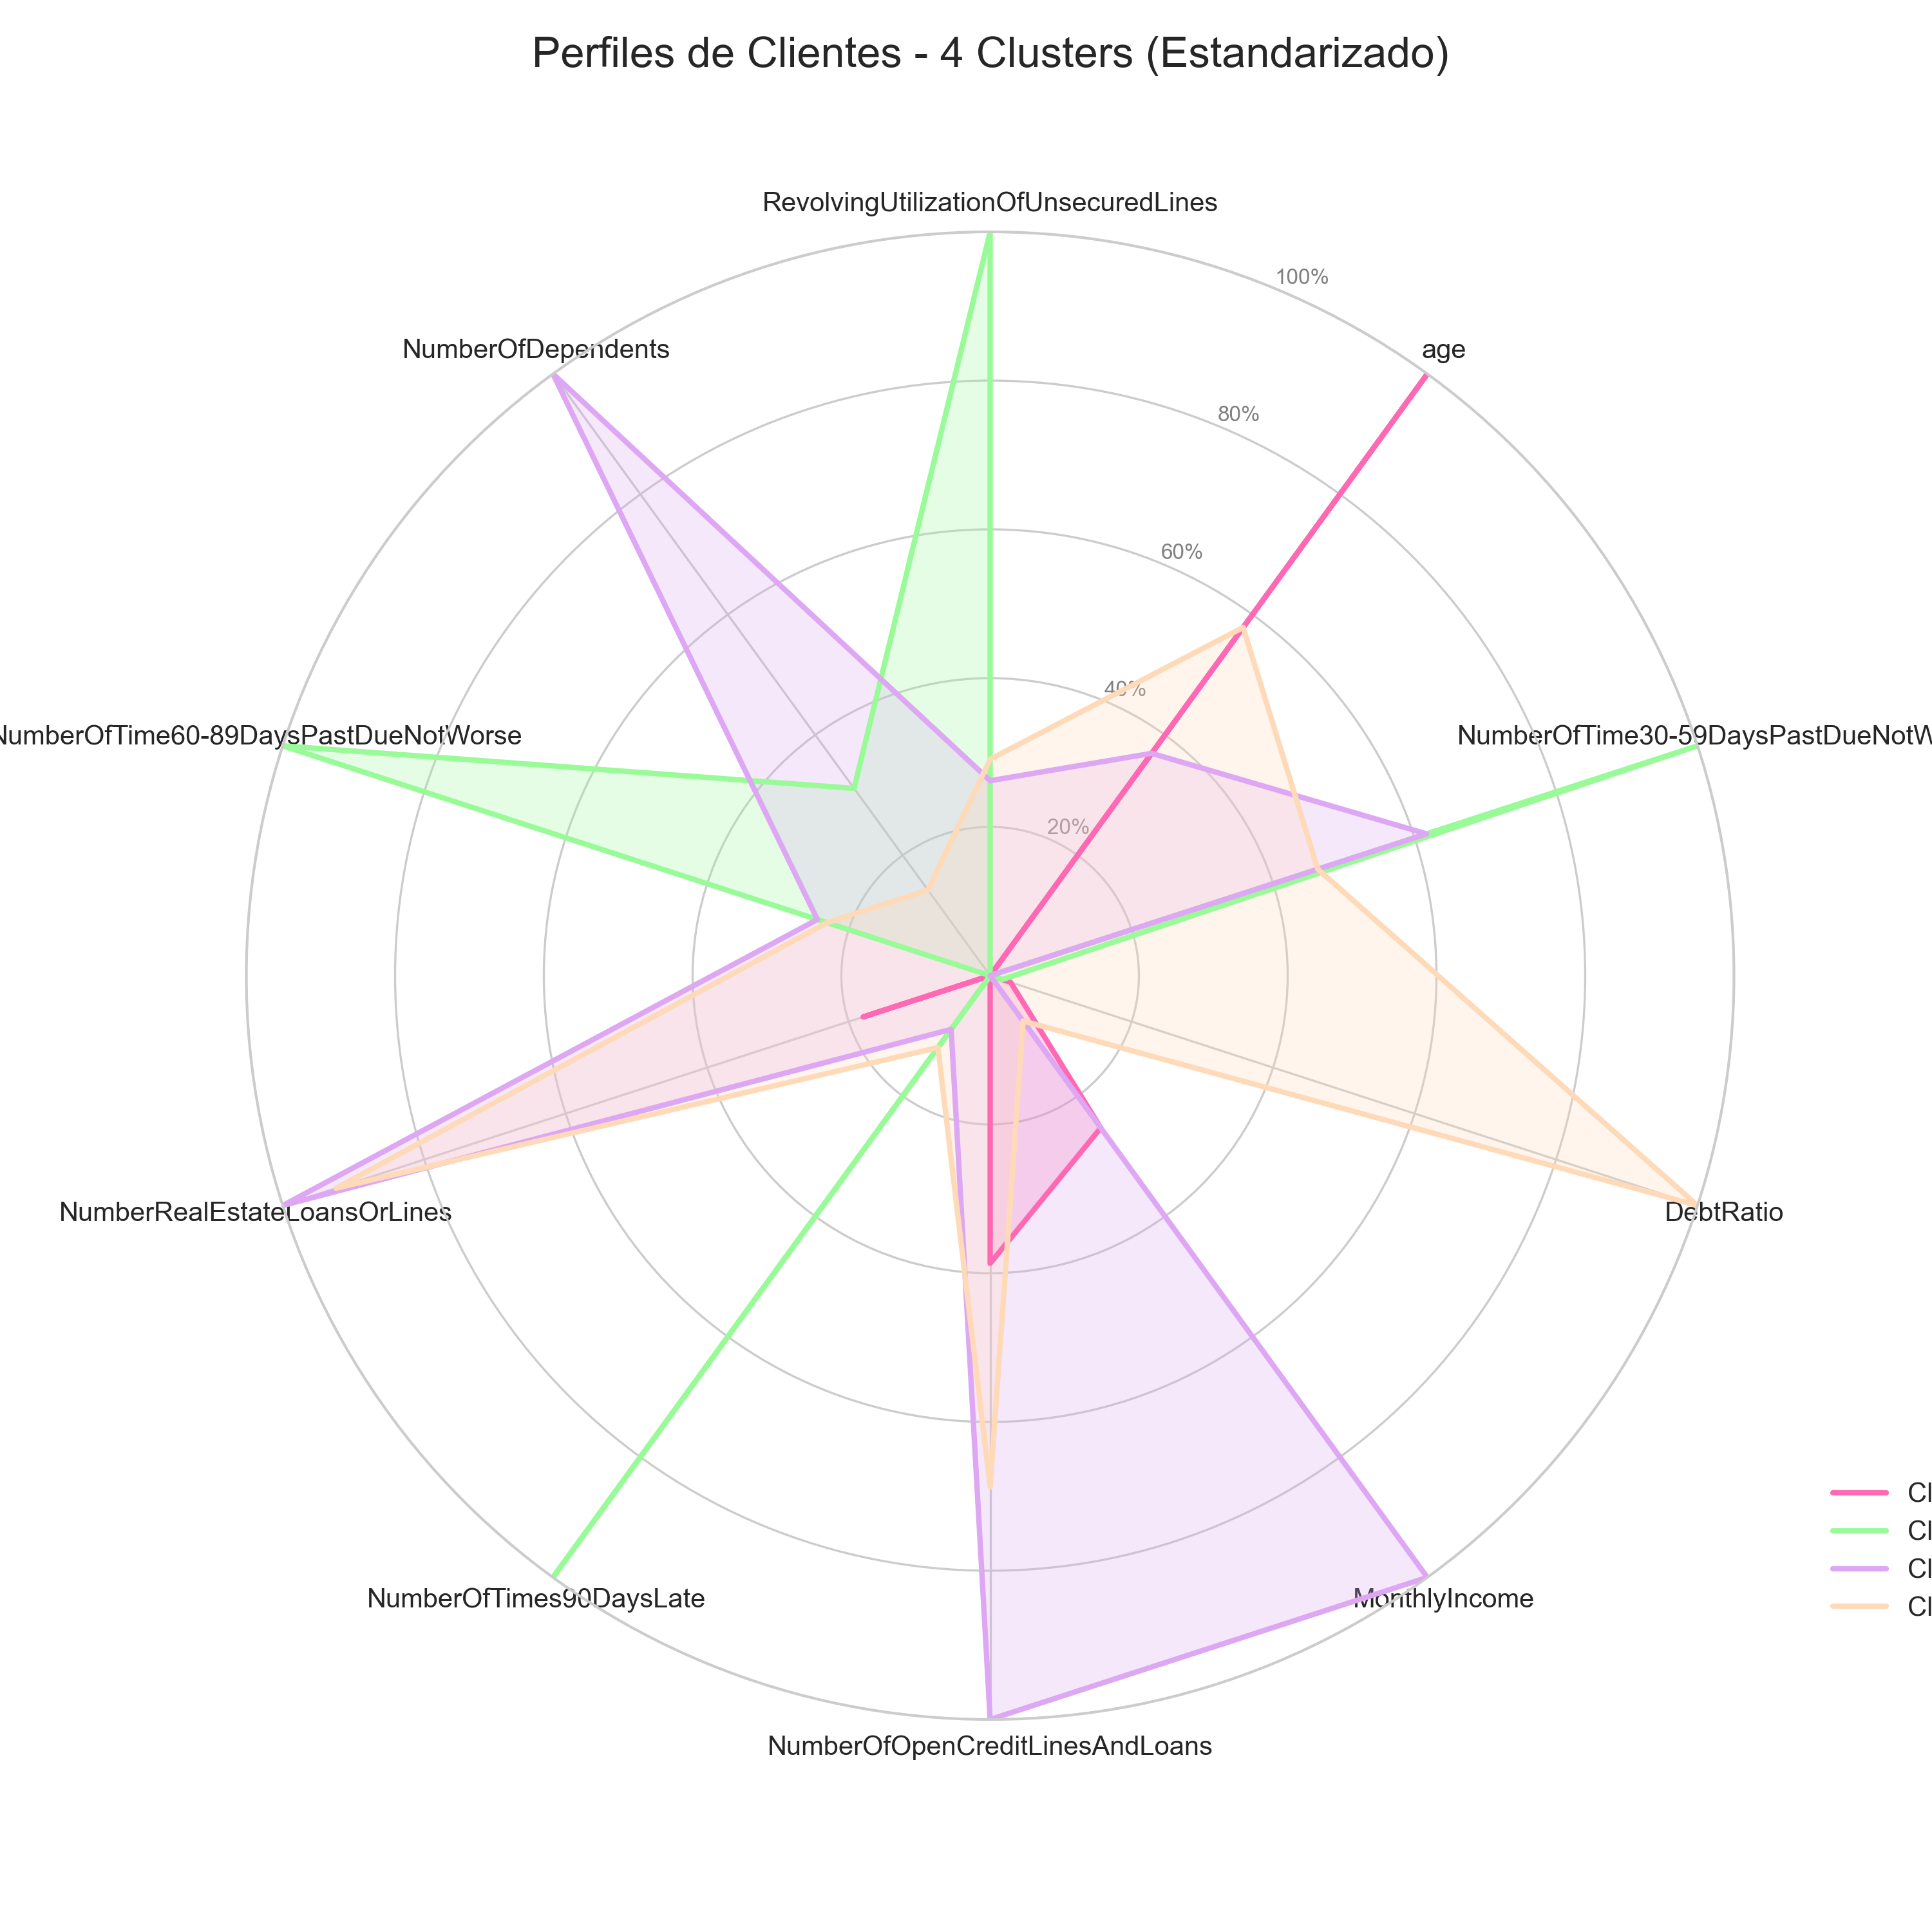
\includegraphics[width=0.8\textwidth]{segmentacion_radar_clusters.png}

\end{frame}

\begin{frame}{\textbf{Interpretación de los perfiles identificados}}

\begin{itemize}
    \item \textcolor{Accent}{\textbf{Cluster 0: Estables y conservadores}}\\
          Baja morosidad, baja utilización del crédito y edad promedio más alta.

    \vspace{0.2cm}
    \item \textcolor{Accent}{\textbf{Cluster 2: Uso intensivo del crédito}}\\
          Mayor utilización del crédito, más dependientes y vulnerabilidad ante cambios en ingresos.

    \vspace{0.2cm}
    \item \textcolor{Accent}{\textbf{Cluster 3: Alta capacidad económica}}\\
          Ingresos más altos, muchas líneas de crédito y varios préstamos inmobiliarios, con morosidad baja.

    \vspace{0.2cm}
    \item \textcolor{Accent}{\textbf{Cluster 4: Sobreendeudados}}\\
          \textit{DebtRatio} extremadamente elevado: gran parte del ingreso se destina al pago de deudas.

    \vspace{0.2cm}
    \item \textcolor{Accent}{\textbf{(Cluster 1: Riesgo extremo, no mostrado en radar)}}\\
          Morosidad muy alta y casi ninguna línea activa; se trata como outlier en algunas visualizaciones.
\end{itemize}

\end{frame}


\begin{frame}{Conclusiones}

\begin{itemize}
    \item La segmentación reveló \textbf{cuatro perfiles financieros claros} en la población:
    estables, vulnerables, alta capacidad y sobreendeudados.
    
    \vspace{0.25cm}
    \item El uso combinado de \textbf{PCA + K-Means} permitió capturar la estructura real del
    conjunto y separar patrones que no son visibles directamente en las variables originales.
    
    \vspace{0.25cm}
    \item El preprocesamiento resultó clave: sin imputación, winsorización y escalado,
    los resultados habrían sido inestables o poco interpretables.
    
    \vspace{0.25cm}
    \item La metodología mostró que los datos financieros contienen \textbf{patrones latentes}
    que pueden ser útiles para análisis de riesgo u orientación de estrategias crediticias.
    
    \vspace{0.25cm}
    \item Como siguiente paso, sería valioso comparar esta segmentación con métodos alternativos
    y analizar cómo evolucionan los perfiles en datos longitudinales.
\end{itemize}

\end{frame}


\end{document}
